%% ============================================================================
%%
%%  Master's thesis
%%
%%  Author: FORNAVN EFTERNAVN
%%
%%  Front page, abstract and colophon
%%
%%  Original template: Jakob Lysgaard Rørsted (Mosumgaard)
%% ============================================================================

% ~~~~~~~~~~~~~~~~~~~~~~~~~~~~~~~~~~~~~~~~~~~~~~~~~~~~~~~~~~~~~~~~~~~~~~~~~~~~~
% The title page and verso (colophon)
% ~~~~~~~~~~~~~~~~~~~~~~~~~~~~~~~~~~~~~~~~~~~~~~~~~~~~~~~~~~~~~~~~~~~~~~~~~~~~~

% Get font-info
\makeatletter
\edef\fontandleading{\@memptsize.0/\the\baselineskip}
\makeatother

\begin{titlingpage}

  % The actual front page (corrected for margin displacement)
  \newlength{\frontpagecorrection}
  \calccentering{\frontpagecorrection}
  \begin{adjustwidth*}{\frontpagecorrection-2cm}{-\frontpagecorrection-2cm}

    \centering
    \scshape

    {\fontsize{33pt}{39pt}\selectfont\spread{\textsc{APODORA}:}} \par
    \vspace{0.3cm}
    {\fontsize{22pt}{26pt}\selectfont\spread{ A Novel Code for Describing}} \par
    \vspace{0.15cm}
    {\fontsize{22pt}{26pt}\selectfont\spread{Big Bang Nucleosynthesis}} \par
      %\textsc{Apodora}
    \vspace{1.5cm}
    {\fontsize{21pt}{27pt}\selectfont\spread{APODORA:}} \par
    \vspace{0.1cm}
    {\fontsize{14pt}{18pt}\selectfont\spread{En ny kode til at beskrive Big Bang Kernesyntese}} \par%l{\o}se

    %\vspace{2cm}
    \vspace{1cm}
    %
\includegraphics[height=7cm]{front/segla1b}
    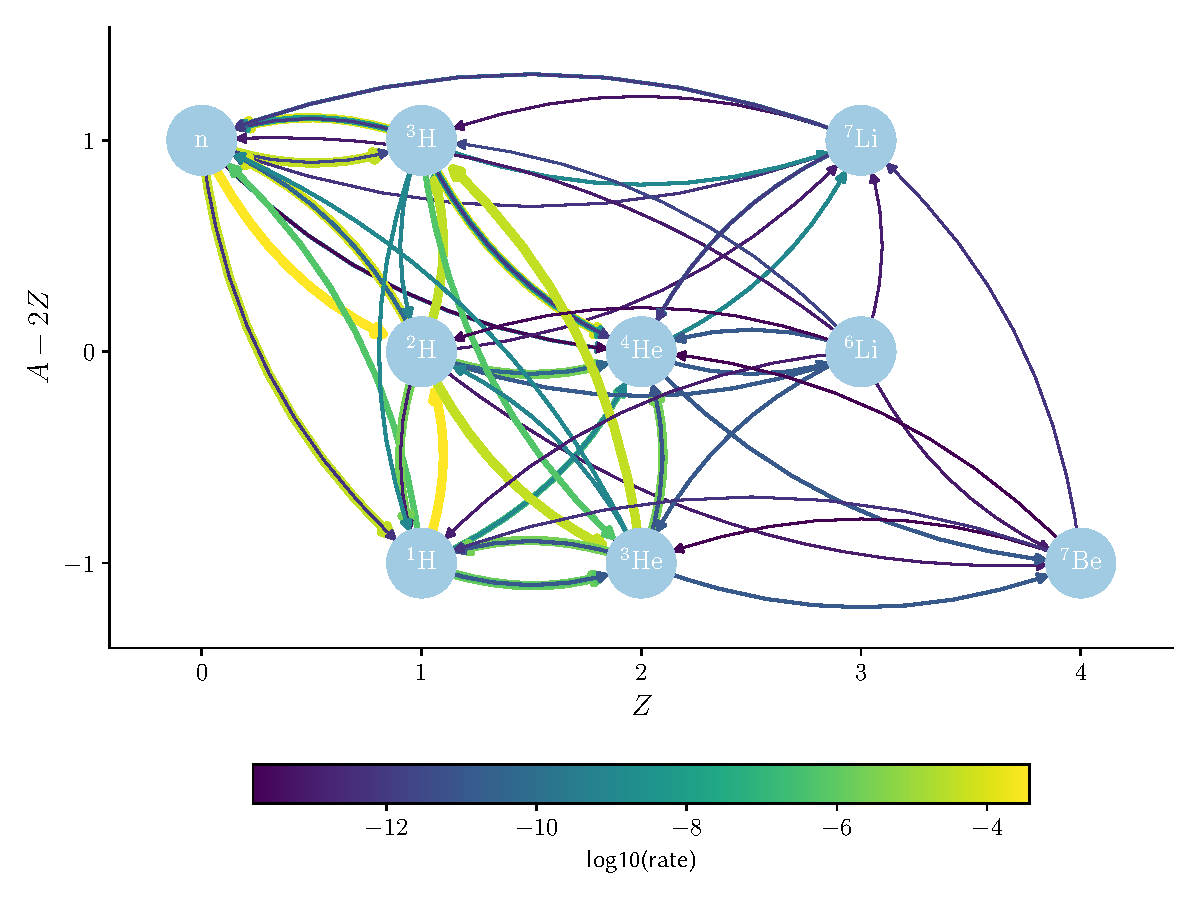
\includegraphics[height=10cm,trim={2cm 4.5cm 1cm 0},clip]{figures/smallnet5minutes.pdf}

    \vspace{1cm}

    \fontsize{16pt}{20pt}\selectfont
    \spread{Hans Br{\"u}ner Dein}\par
    \spread{201706079}\par

    \bigskip

    \fontsize{14pt}{18pt}\selectfont
    \spread{Master's Thesis in Physics}\par
    \spread{February 2024}\par
    %\bigskip
    \vfill

    Supervisors: Thomas Tram \& Steen Hannested\par
    % \href{http://pure.au.dk/portal/da/persons/id(XXX).html}{NAVN} \par

    \vfill

    \fontsize{12pt}{14.5pt}\selectfont
    \href{https://www.phys.au.dk/}{Department of Physics and Astronomy}\par
    \href{https://www.au.dk/}{Aarhus University}

  \end{adjustwidth*}

  % Colophon
  \newpage
  \begin{adjustwidth*}{\frontpagecorrection}{-\frontpagecorrection}
    \thispagestyle{empty}
    \strut\vfill
    {
      \setlength{\parindent}{0pt}
      \addtolength{\parskip}{.6em}

      \begin{center}
        \bfseries\sffamily Colophon
      \end{center}

      \small

      \textsl{\projecttitle}

      {--- \textsl{\projecttitledanish}}

      \smallskip

      Master's thesis by Hans Br{\"u}ner Dein. Written under supervision by Asc.Prof. Thomas Tram \& Prof. Steen Hannested
      Department of Physics and Astronomy, Aarhus University.

      Typeset by the author with \LaTeX{} and the \textsf{memoir} document class,
      using Linux Libertine and Linux Biolinum {\fontandleading}.

      Printed at Aarhus University
    }
  \end{adjustwidth*}
\end{titlingpage}


% ~~~~~~~~~~~~~~~~~~~~~~~~~~~~~~~~~~~~~~~~~~~~~~~~~~~~~~~~~~~~~~~~~~~~~~~~~~~~~
% Abstracts
% ~~~~~~~~~~~~~~~~~~~~~~~~~~~~~~~~~~~~~~~~~~~~~~~~~~~~~~~~~~~~~~~~~~~~~~~~~~~~~
\thispagestyle{chapter}

% ~~~~~~~~~~~~~~~~~
% Abstract: English
% ~~~~~~~~~~~~~~~~~
\begin{multiabstract}{Abstract (English)} 
\noindent The goal of this thesis is to present the development of a new BBN code APODORA (Adaptable Python interface Offering Determination Of Relic Abundances). APODORA is designed to be more flexible than existing codes, with an emphasis on the use of modern standardized computing methods. Derivations of the equations describing the time evolution of various components in the early universe are presented. These are implemented in a flexible IPython environment with the reaction network being created using interfaces from pynucastro\cite{pynucastro2}. The numerical uncertainty associated with every relevant input parameter of the code is systematically examined to ensure a high level of numerical precision. An in-depth comparison between APODORA and \textsc{AlterBBN} is performed, demonstrating equal or superior precision and speed. Finally, the resulting final abundances from APODORA are compared with multiple existing BNN codes as well as observational data.

\end{multiabstract}


% ~~~~~~~~~~~~~~~~~
% Abstract: Danish
% ~~~~~~~~~~~~~~~~~
\plainbreak{2}

% Switch to Danish
\selectlanguage{danish}
\begin{multiabstract}{Resumé (Dansk)}
\noindent Målet med dette speciale er at præsentere udviklingen af en ny BBN-kode APODORA, (Adaptable Python interface Offering Determination Of Relic Abundances). APODORA er skabt med henblik på at være mere fleksible end eksisterende løsninger, men særlig fokus på anvendelsen af moderne og standardiserende løsningsmetoder. Udledning af ligningerne som beskriver tidsudviklingen af det tidlige univers bestanddele bliver præsenteret. Dette er implementeret i et fleksibelt IPython miljø, hvortil reaktionsnetværket bliver skabt ved hjælp af brugerflader fra pakken pynucastro\cite{pynucastro2}. Den numeriske usikkerhed forbundet med hver relevant inputparameter i koden undersøges systematisk, for at sikre et højt niveau af numerisk præcision. Der udføres en dybdegående sammenligning af APODORA og \textsc{AlterBBN}, som viser at både hastighed og præcision er lige så god, hvis ikke bedre. Til sidst sammenlignes forudsigelserne fra APODORA med andre BNN-koder samt observationer.

\end{multiabstract}

% Reset document language to English
\selectlanguage{english}